\chapter{Diseño de circuito impreso} \chapterlabel{Informe/8-PCB} \label{cap:PCB}


En este capítulo se muestran los esquemáticos y las imágenes del PCB desarrollados para la implementación de la placa de control. 

Por otra parte, se describen las consideraciones y circuitos utilizados para las fuentes de alimentación del sistema.


\section{Fuentes de Alimentación}

\subsection{Fuente de alimentación externa de $24\:V$}

\noindent La fuente externa se encarga de alimentar todo el circuito. Debe ser capaz de suministrar $24\:V$ y hasta $30\:A$. Para ello se puede utilizar una fuente de laboratorio o baterías.

\subsection{Fuente de alimentación interna de $12\:V$}

\noindent La fuente de $12\:V$ se encarga de alimentar al regulador de $5\:V$ y al driver del puente H. Debido a los bajos consumos de potencia y bajo costo, se utiliza una fuente lineal. Por lo tanto, se decide utilizar el integrado L78M12CDT-TR.

\subsection{Fuente de alimentación interna de $5\:V$}

La fuente de $5\:V$ se encarga de alimentar los operacionales, el sensor de efecto hall, el inversor y el regulador de tensión de $2.5\:V$. Debido a los bajos consumos de potencia y bajo costo, se utiliza una fuente lineal. Por lo tanto, se decide utilizar el integrado L78M05CDT.

\section{Esquemáticos}

\subsection{Principal}
\begin{figure}[H]
	\centering
	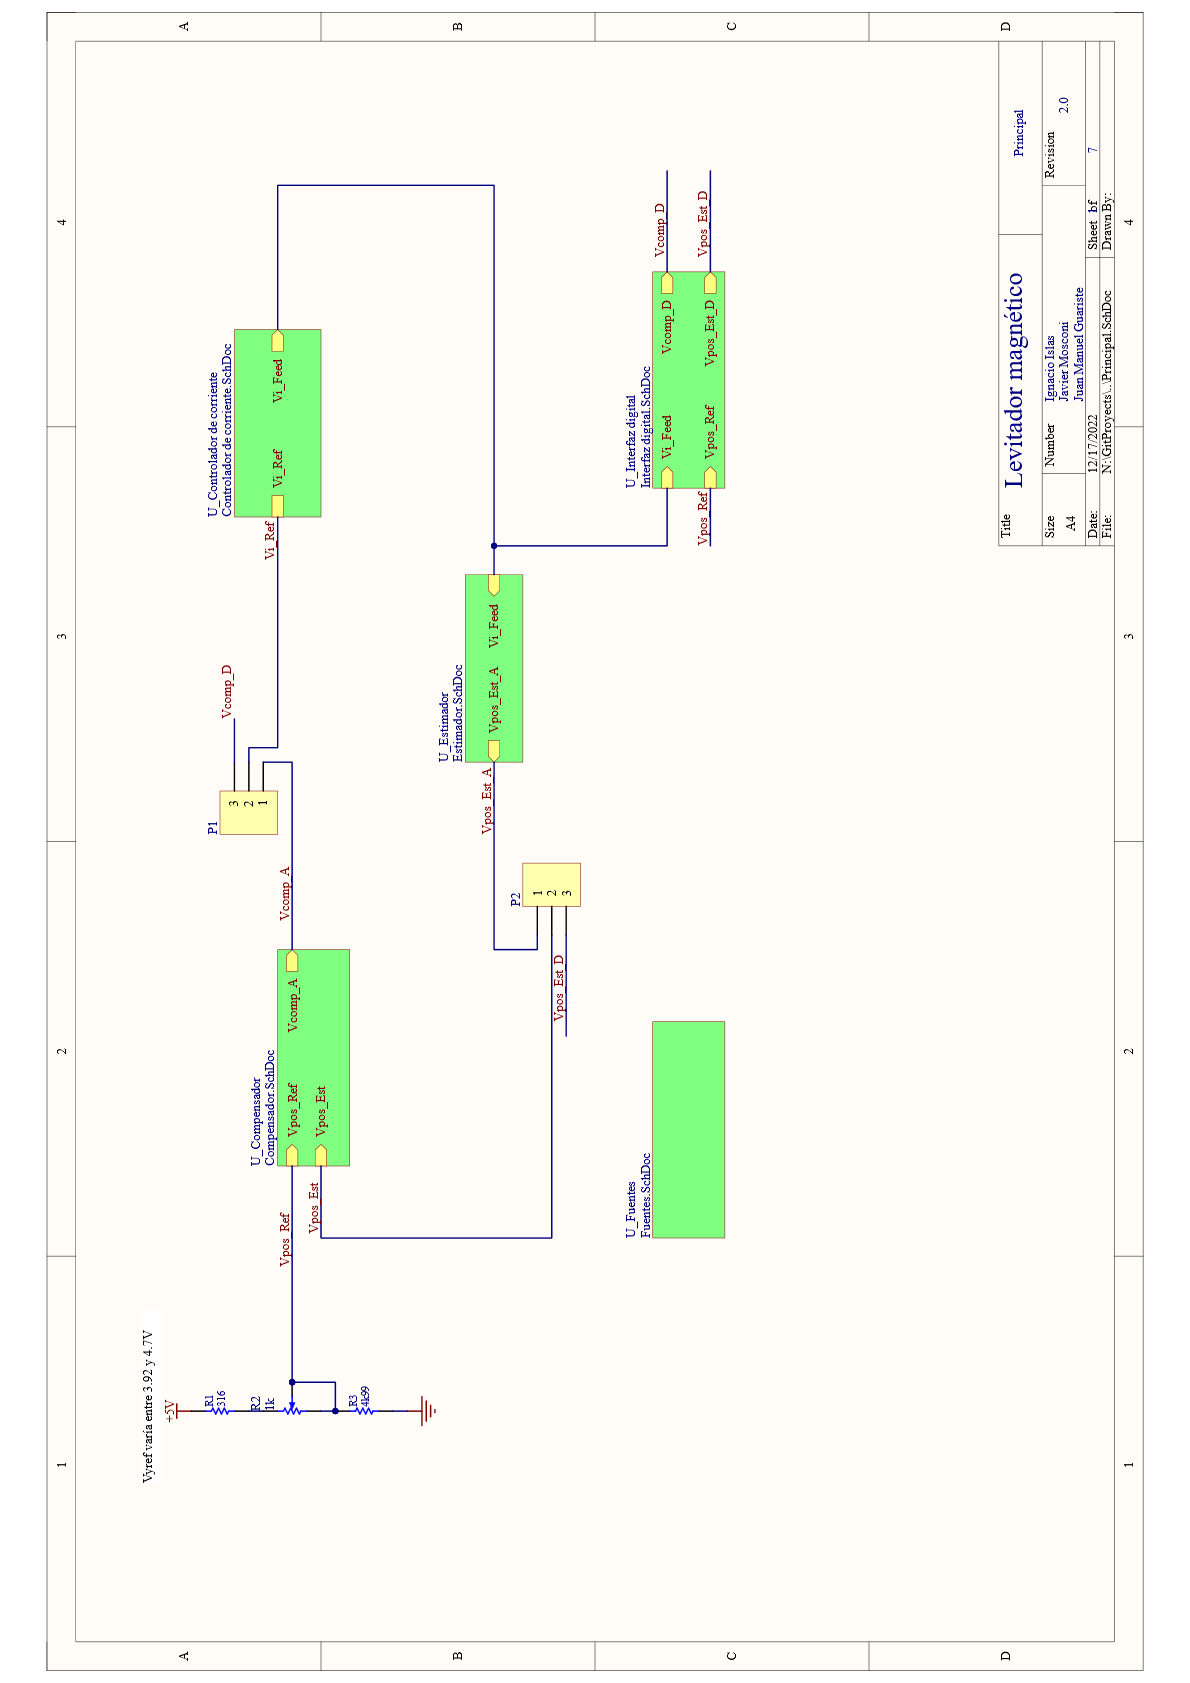
\includegraphics[scale=0.3]{main.png}
	%\caption{Diagrama en bloques de la implementación digital.}
	\label{fig:main}
\end{figure}

\subsection{Controlador de corriente}
\begin{figure}[H]
	\centering
	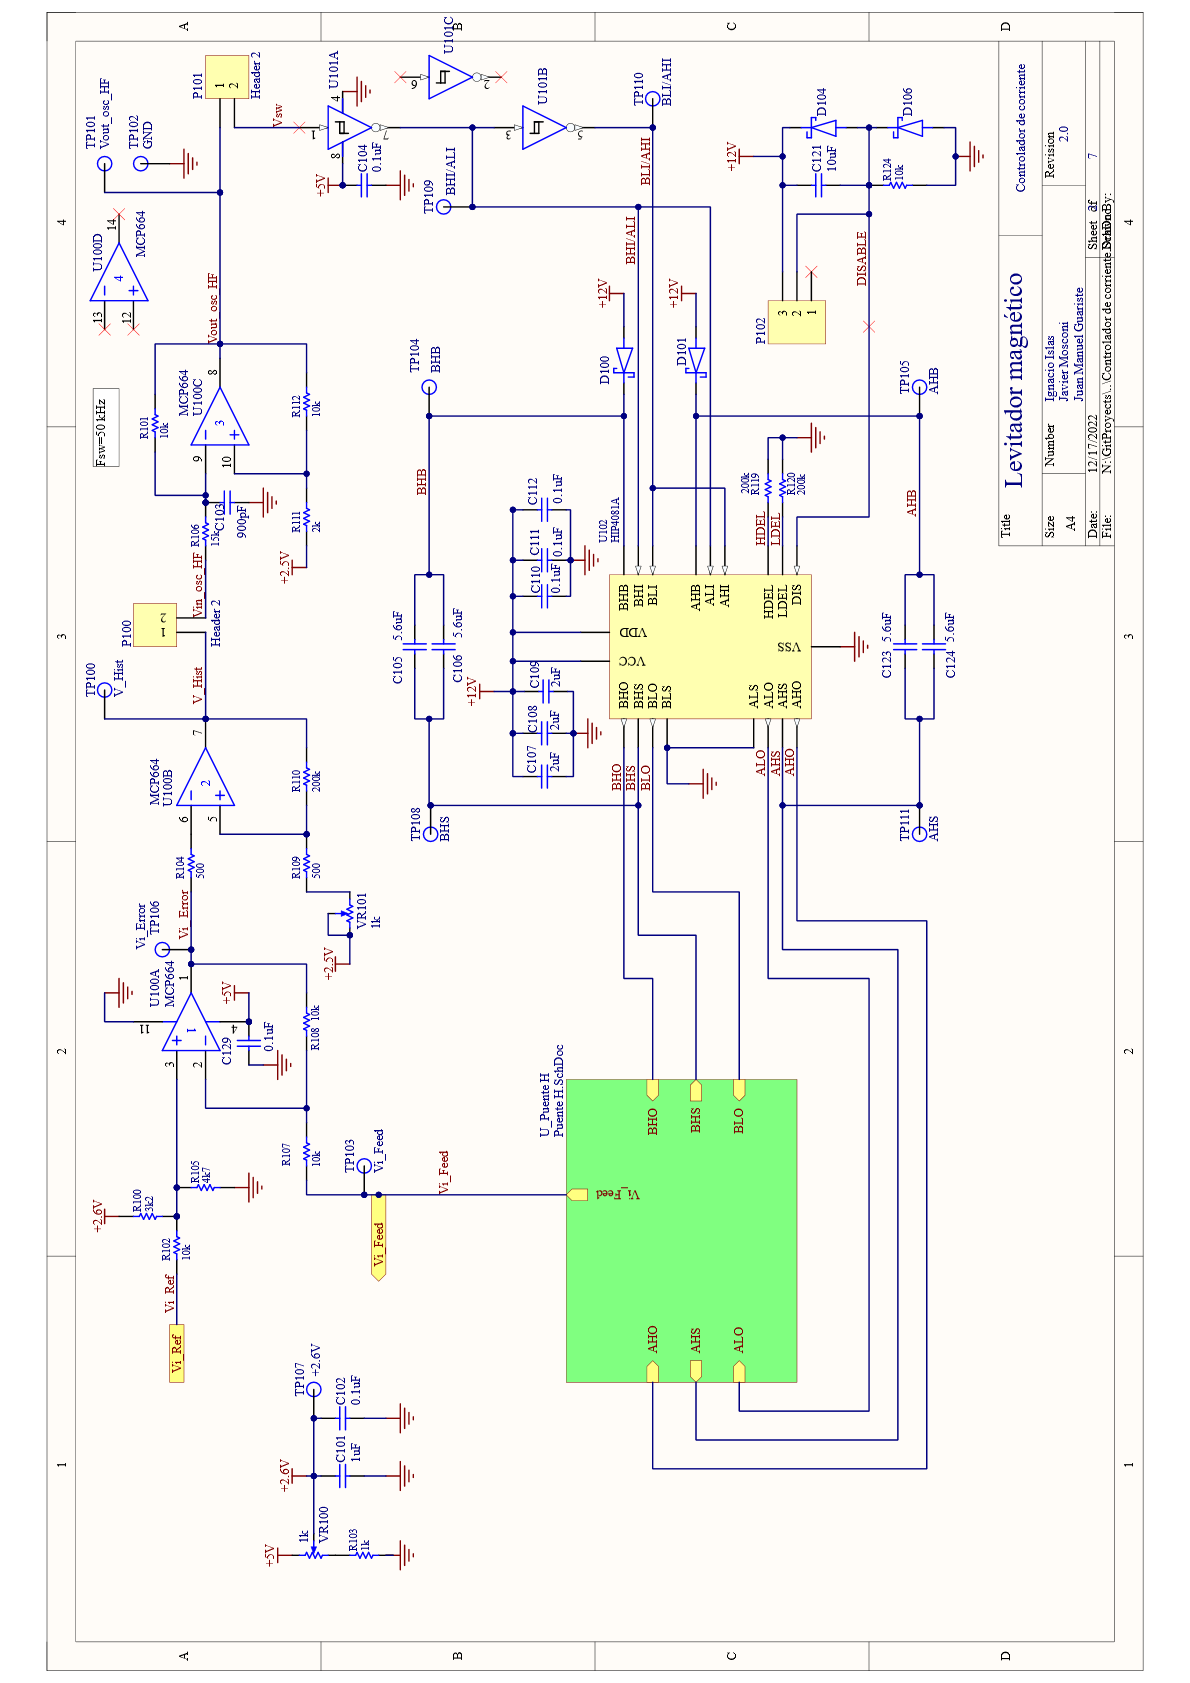
\includegraphics[scale=0.32]{contCorrEsq.png}
	%\caption{Diagrama en bloques de la implementación digital.}
	\label{fig:contCorrEsq}
\end{figure}

\subsection{Puente H}
\begin{figure}[H]
	\centering
	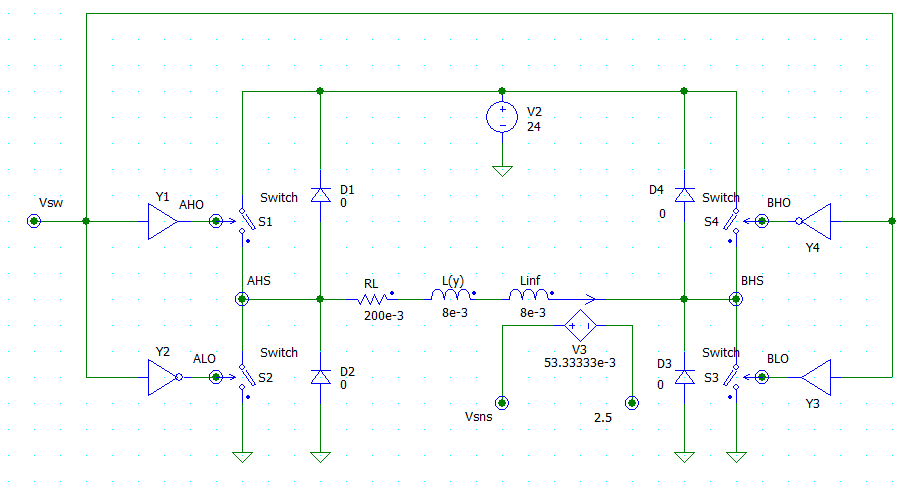
\includegraphics[scale=0.32]{PuenteH.png}
	%\caption{Diagrama en bloques de la implementación digital.}
	\label{fig:PuenteH}
\end{figure}

\subsection{Compensador analógico}
\begin{figure}[H]
	\centering
	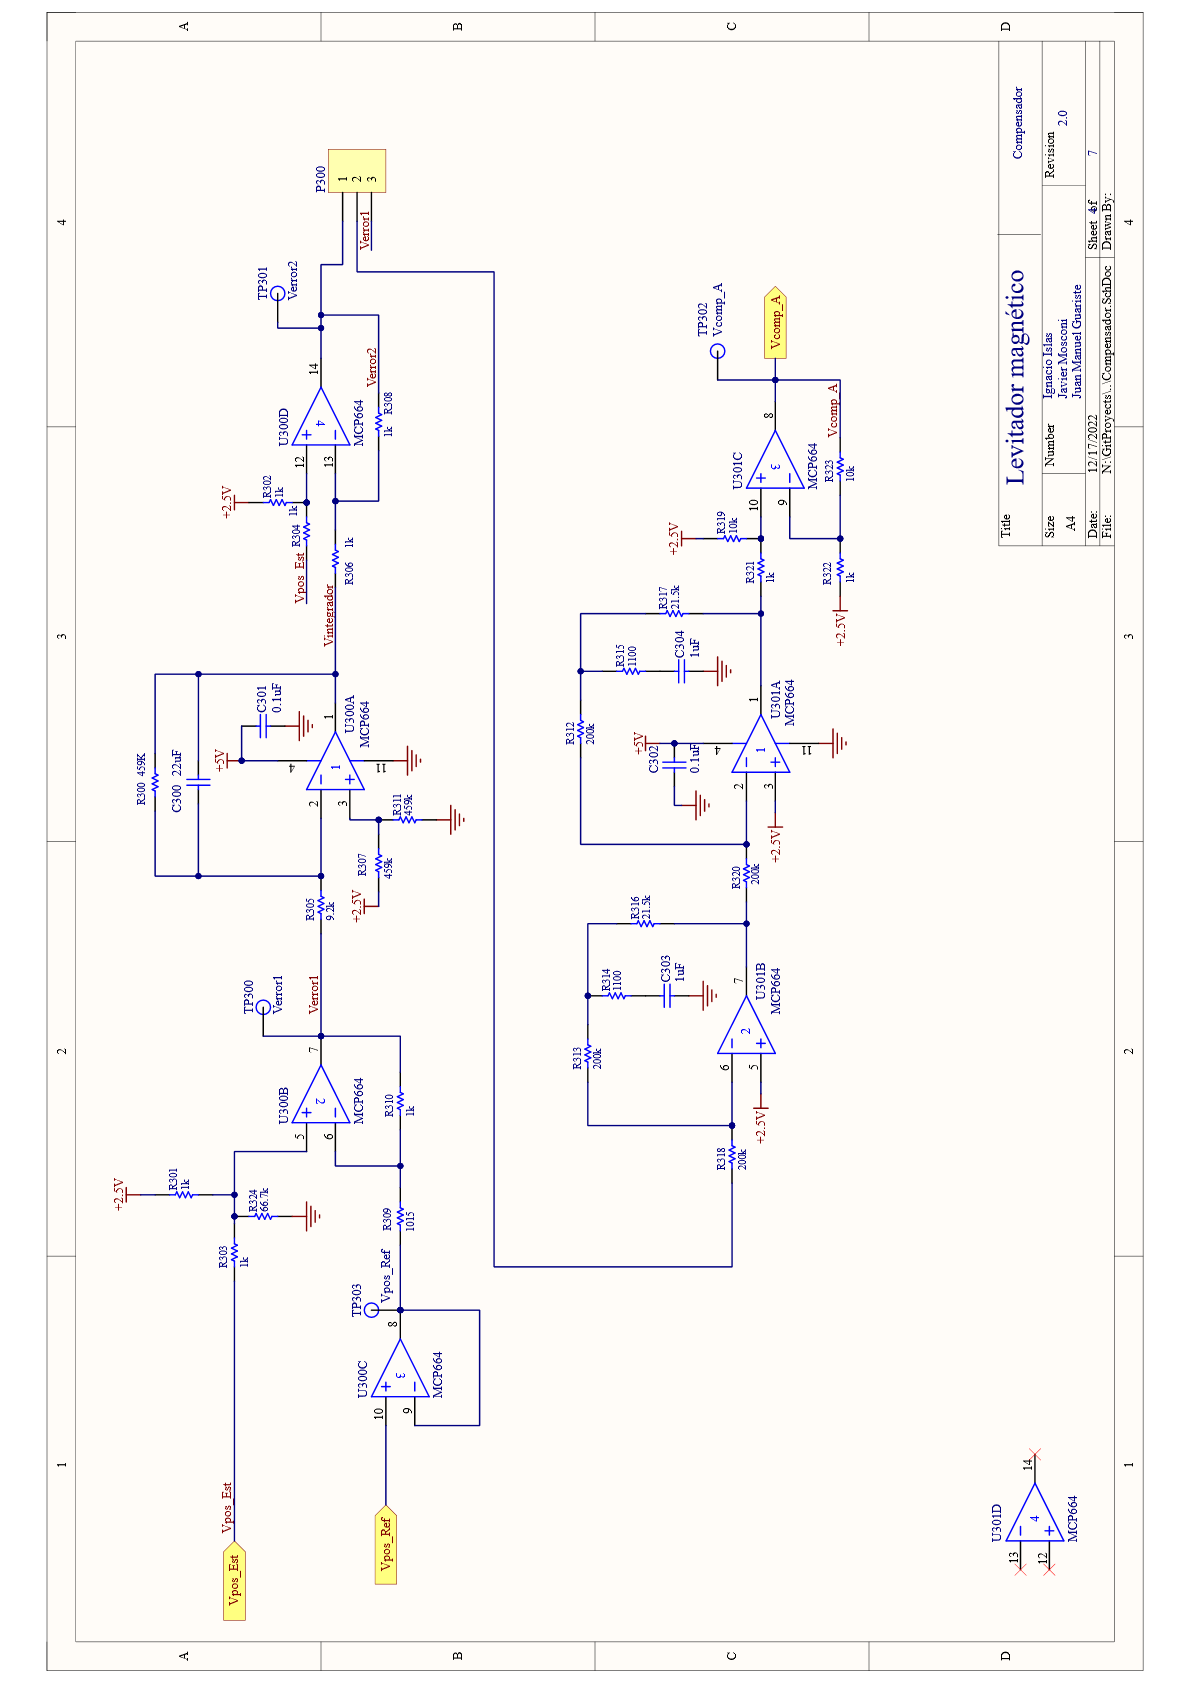
\includegraphics[scale=0.32]{CompAnalog.png}
	%\caption{Diagrama en bloques de la implementación digital.}
	\label{fig:CompAnalog}
\end{figure}

\subsection{Estimador analógico}
\begin{figure}[H]
	\centering
	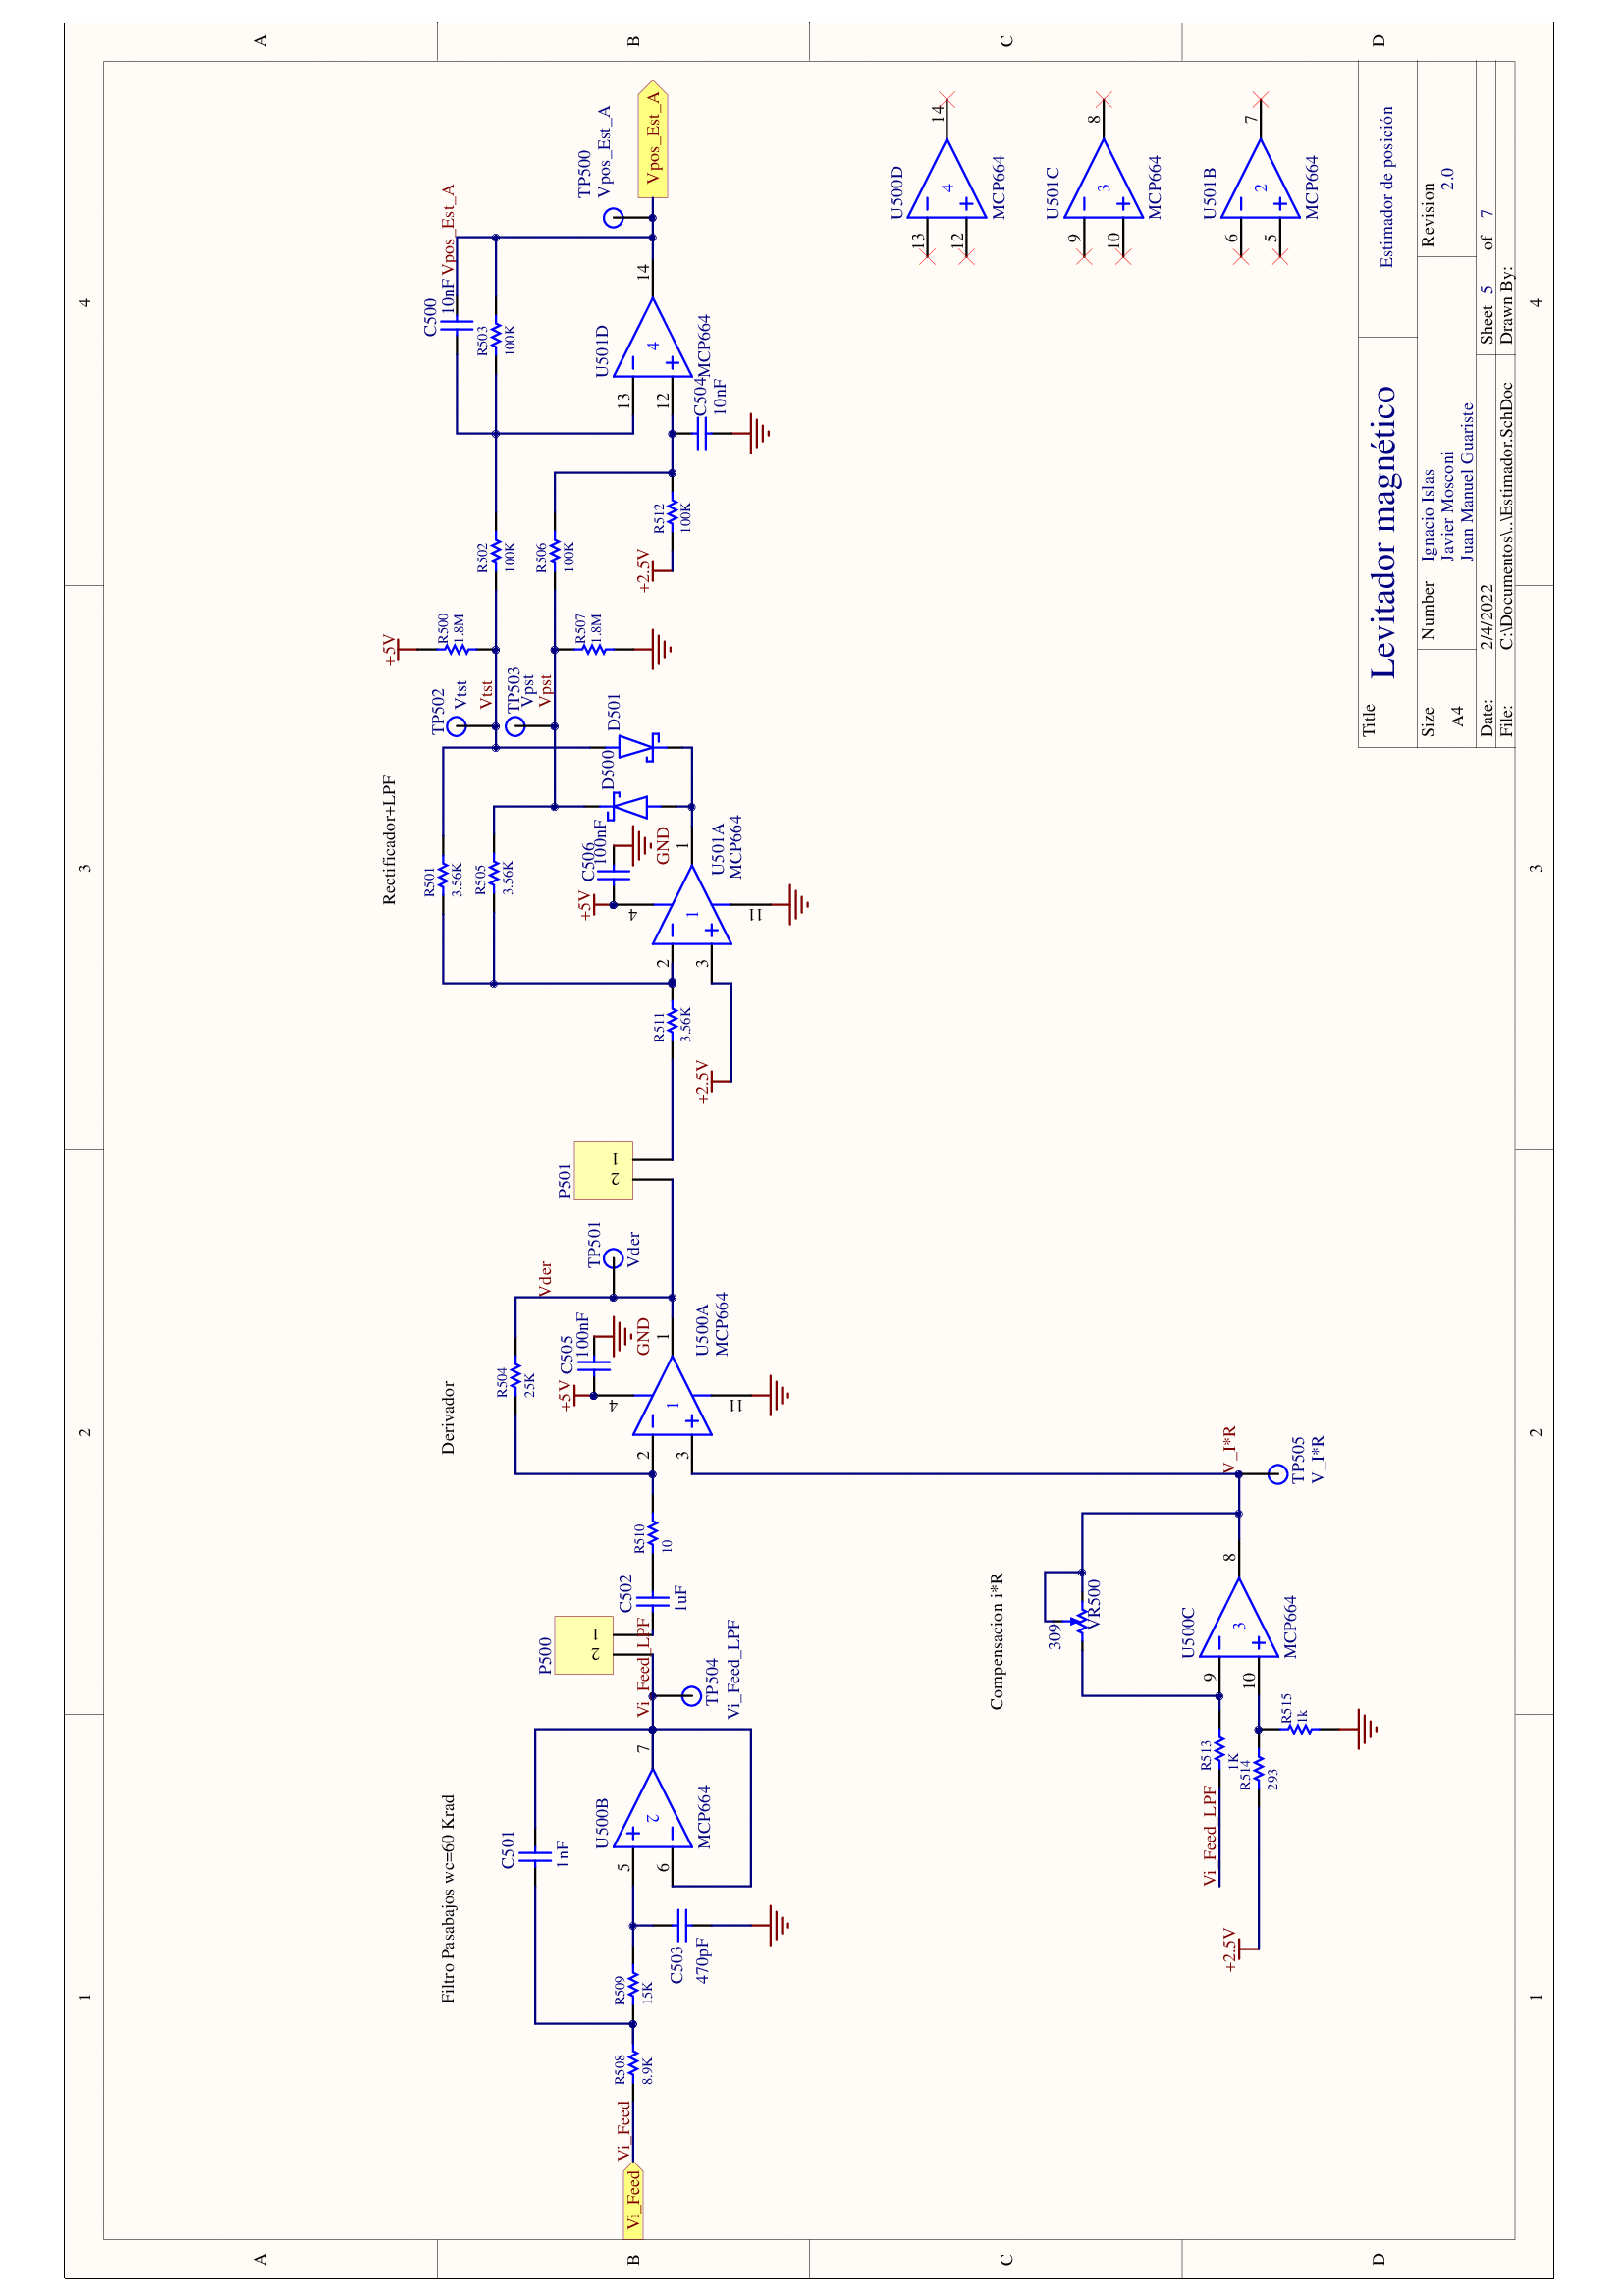
\includegraphics[scale=0.32]{EstimAnalog.png}
	%\caption{Diagrama en bloques de la implementación digital.}
	\label{fig:EstimAnalog}
\end{figure}

\subsection{Interfaz con microcontrolador}
\begin{figure}[H]
	\centering
	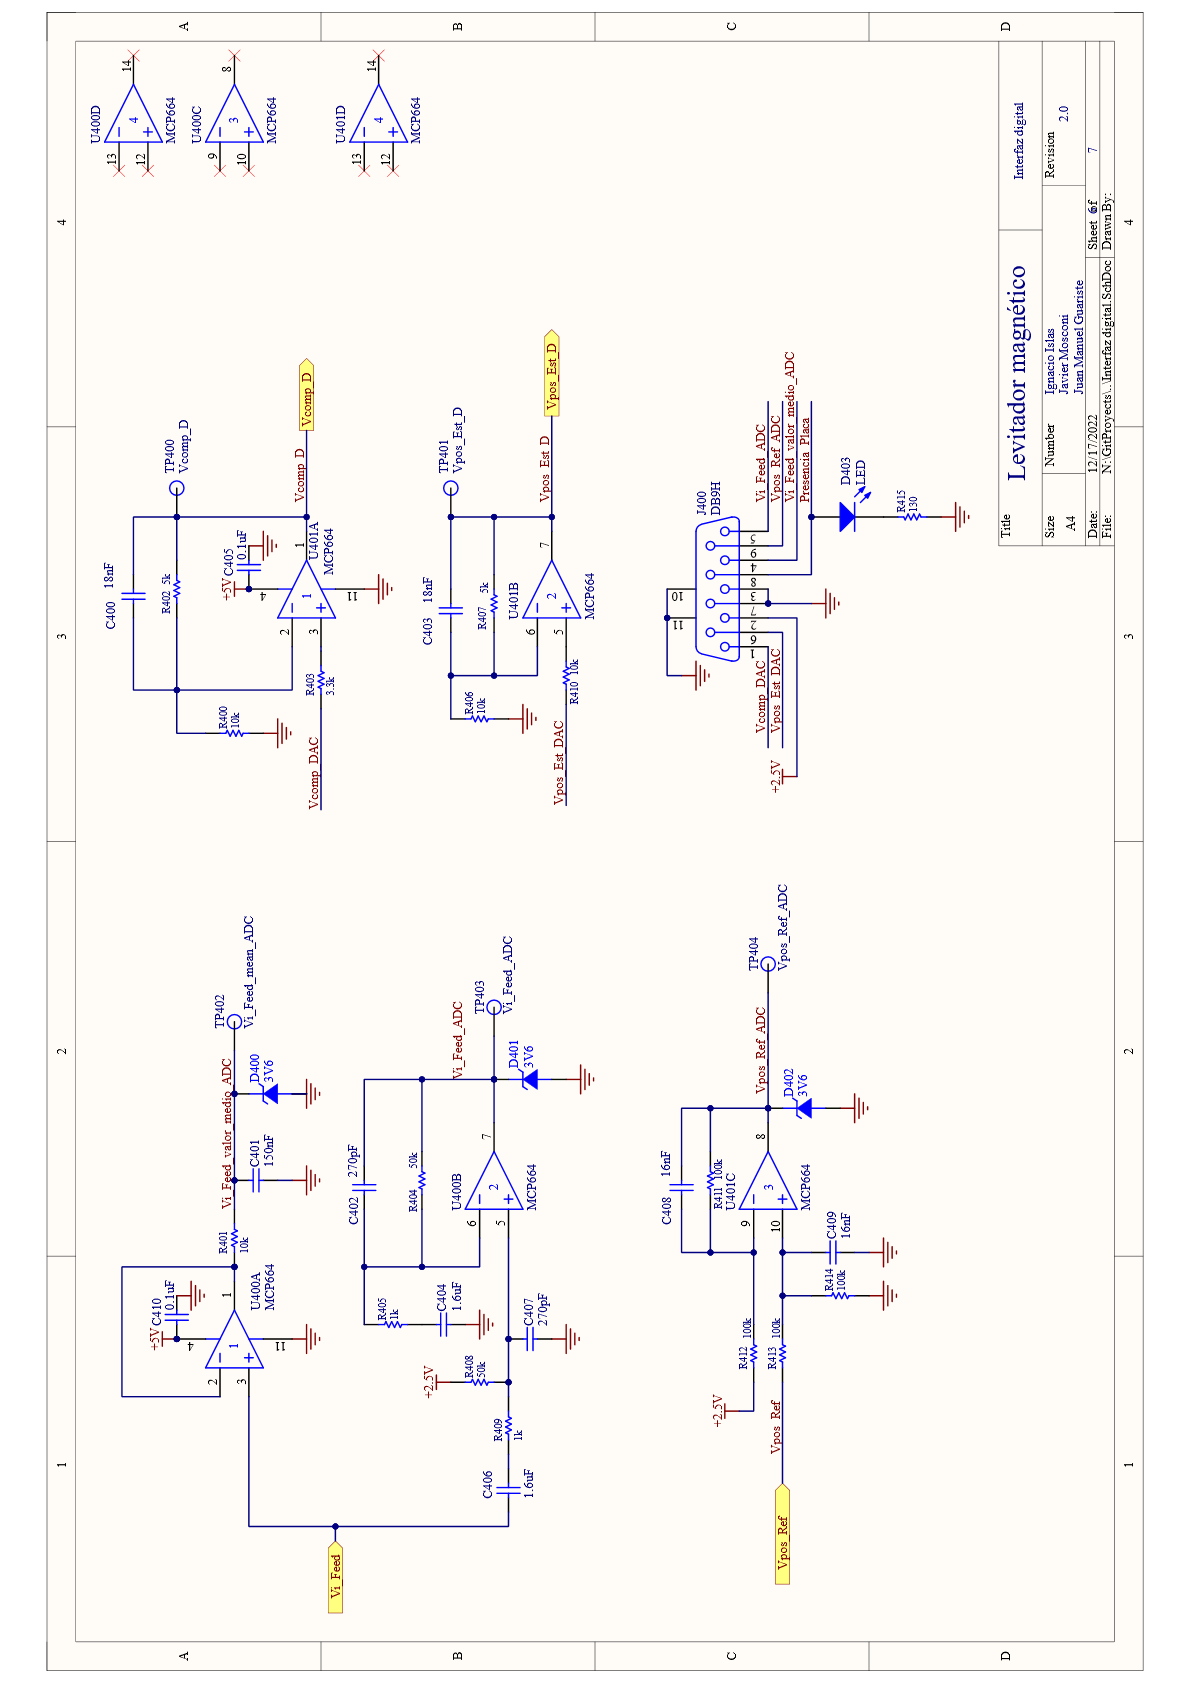
\includegraphics[scale=0.32]{InterfazMic.png}
	%\caption{Diagrama en bloques de la implementación digital.}
	\label{fig:InterfazMic}
\end{figure}

\subsection{Fuentes de alimentación}
\begin{figure}[H]
	\centering
	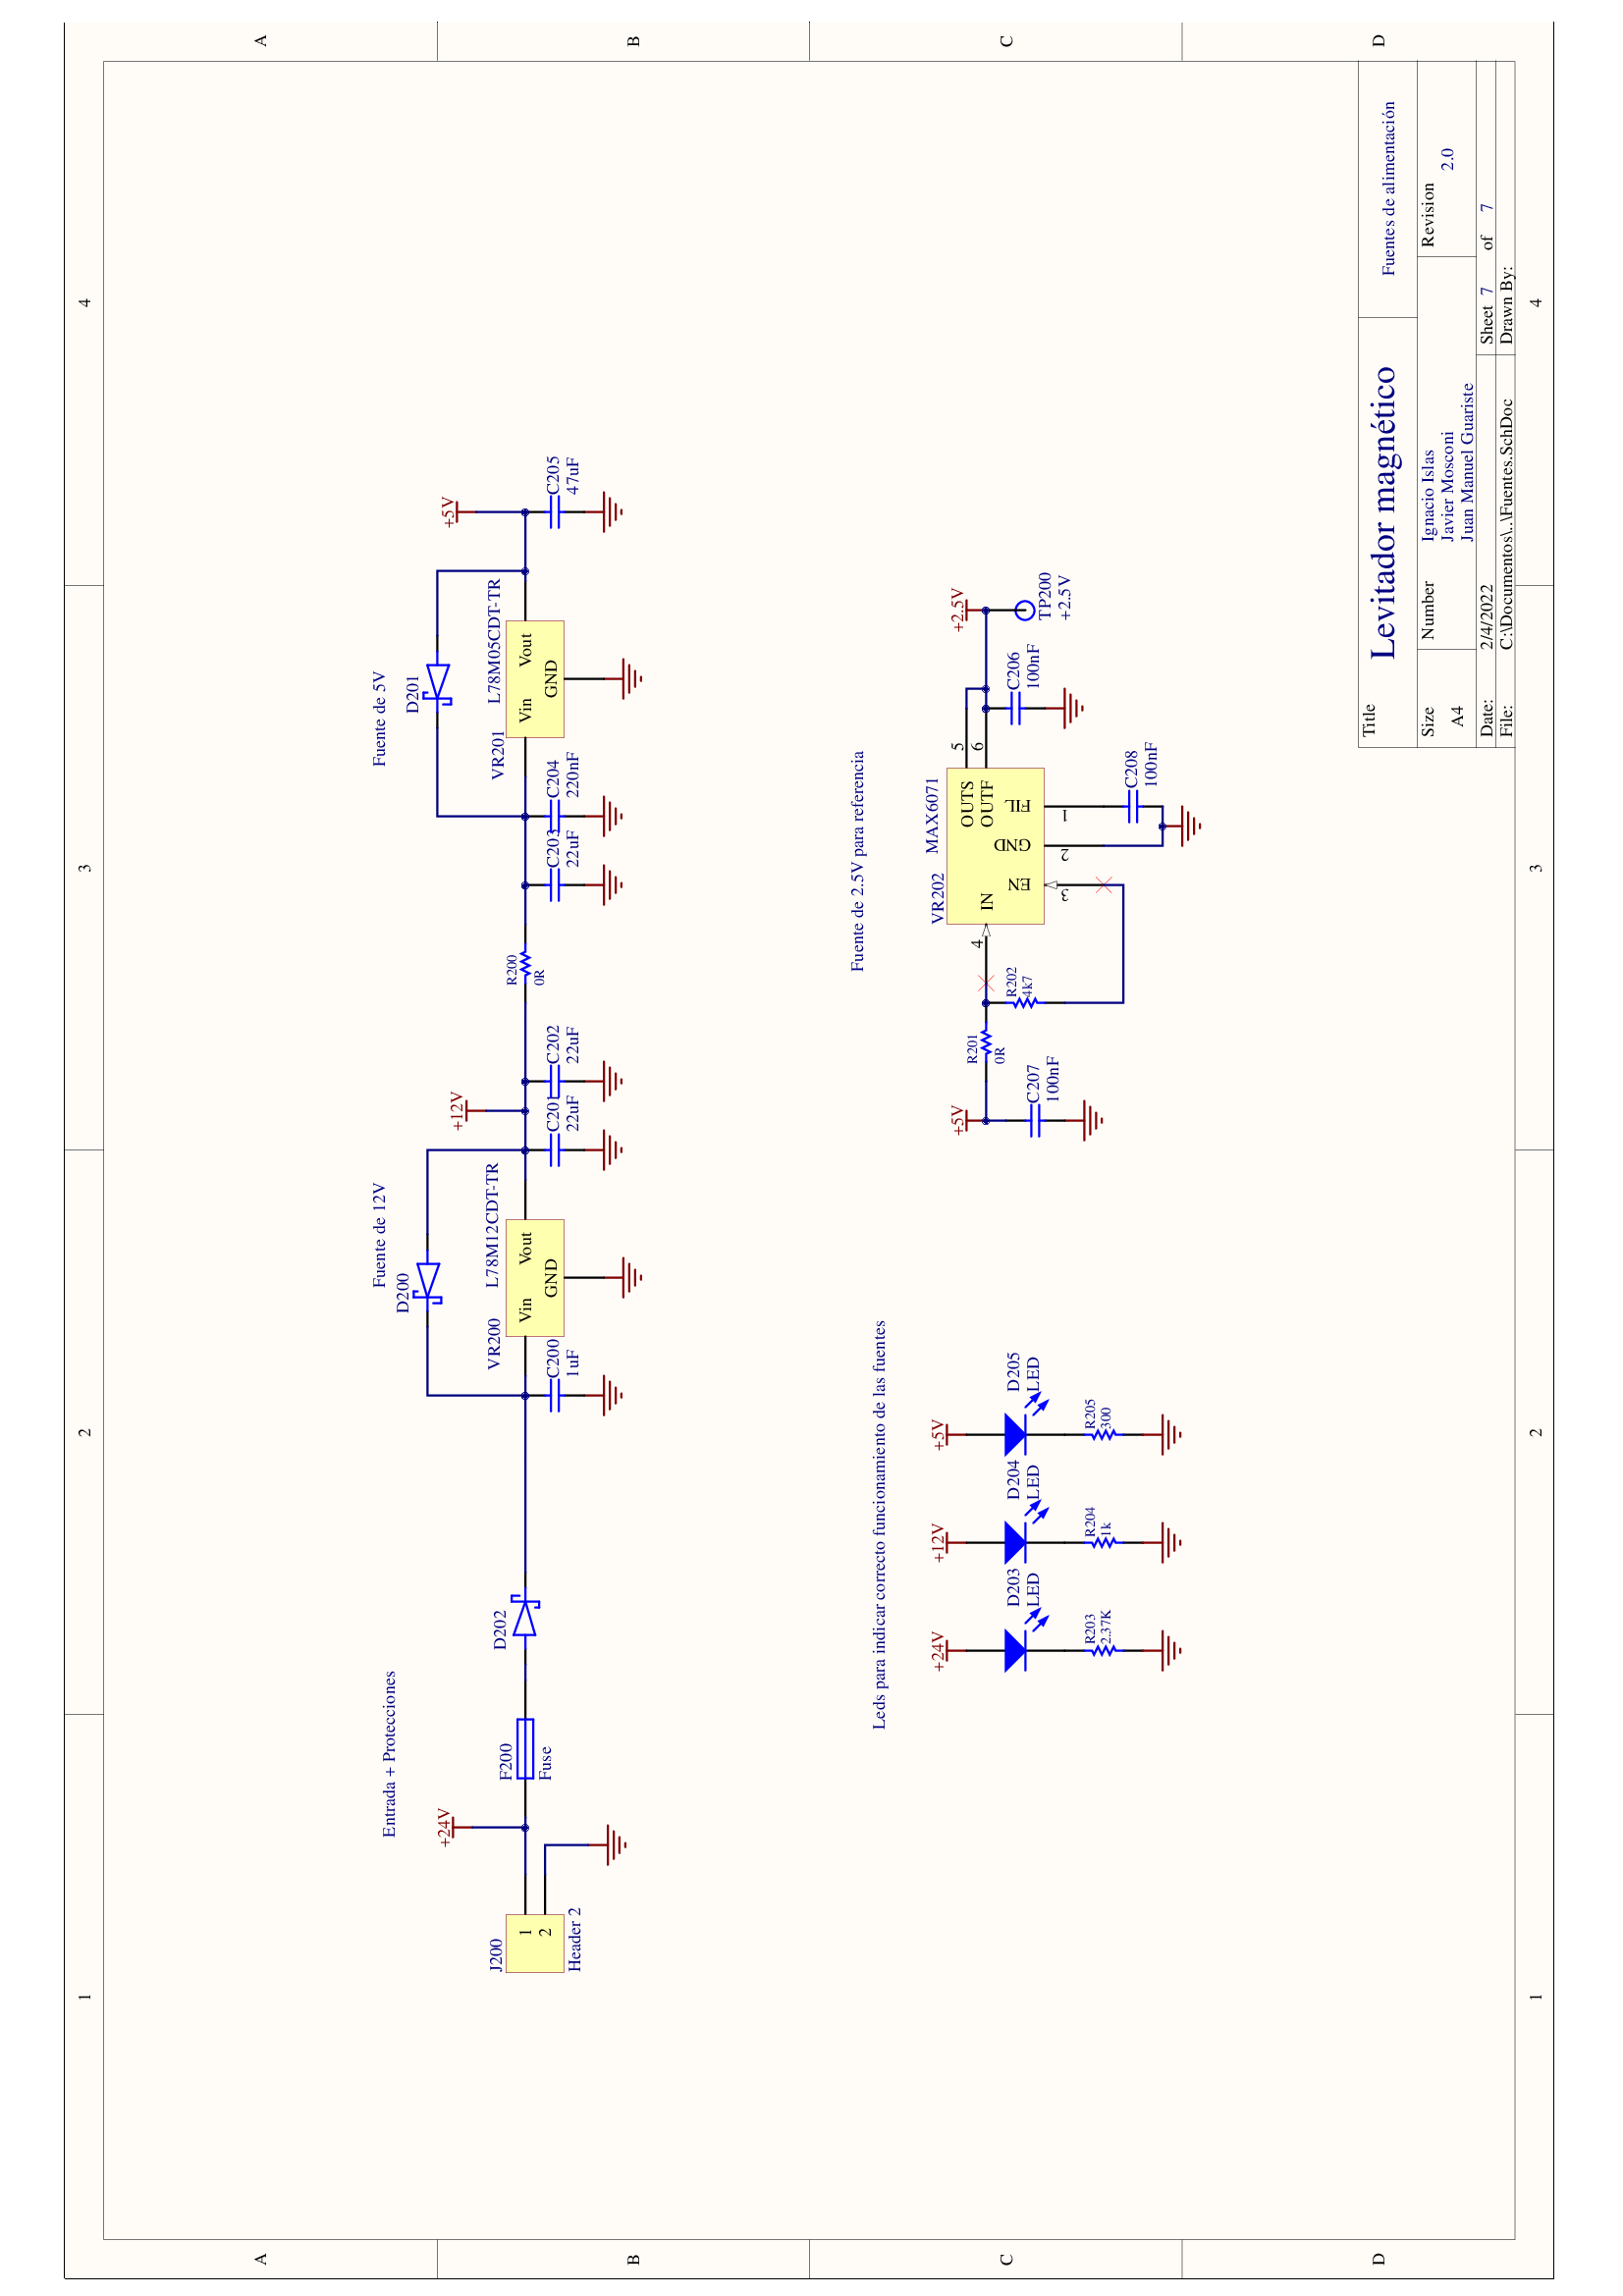
\includegraphics[scale=0.3]{FuentesAliment.png}
	%\caption{Diagrama en bloques de la implementación digital.}
	\label{fig:FuentesAliment}
\end{figure}

\section{PCB}
\subsection{Modelo 2D}
\subsubsection{Vista Superior}
\begin{figure}[H]
	\centering
	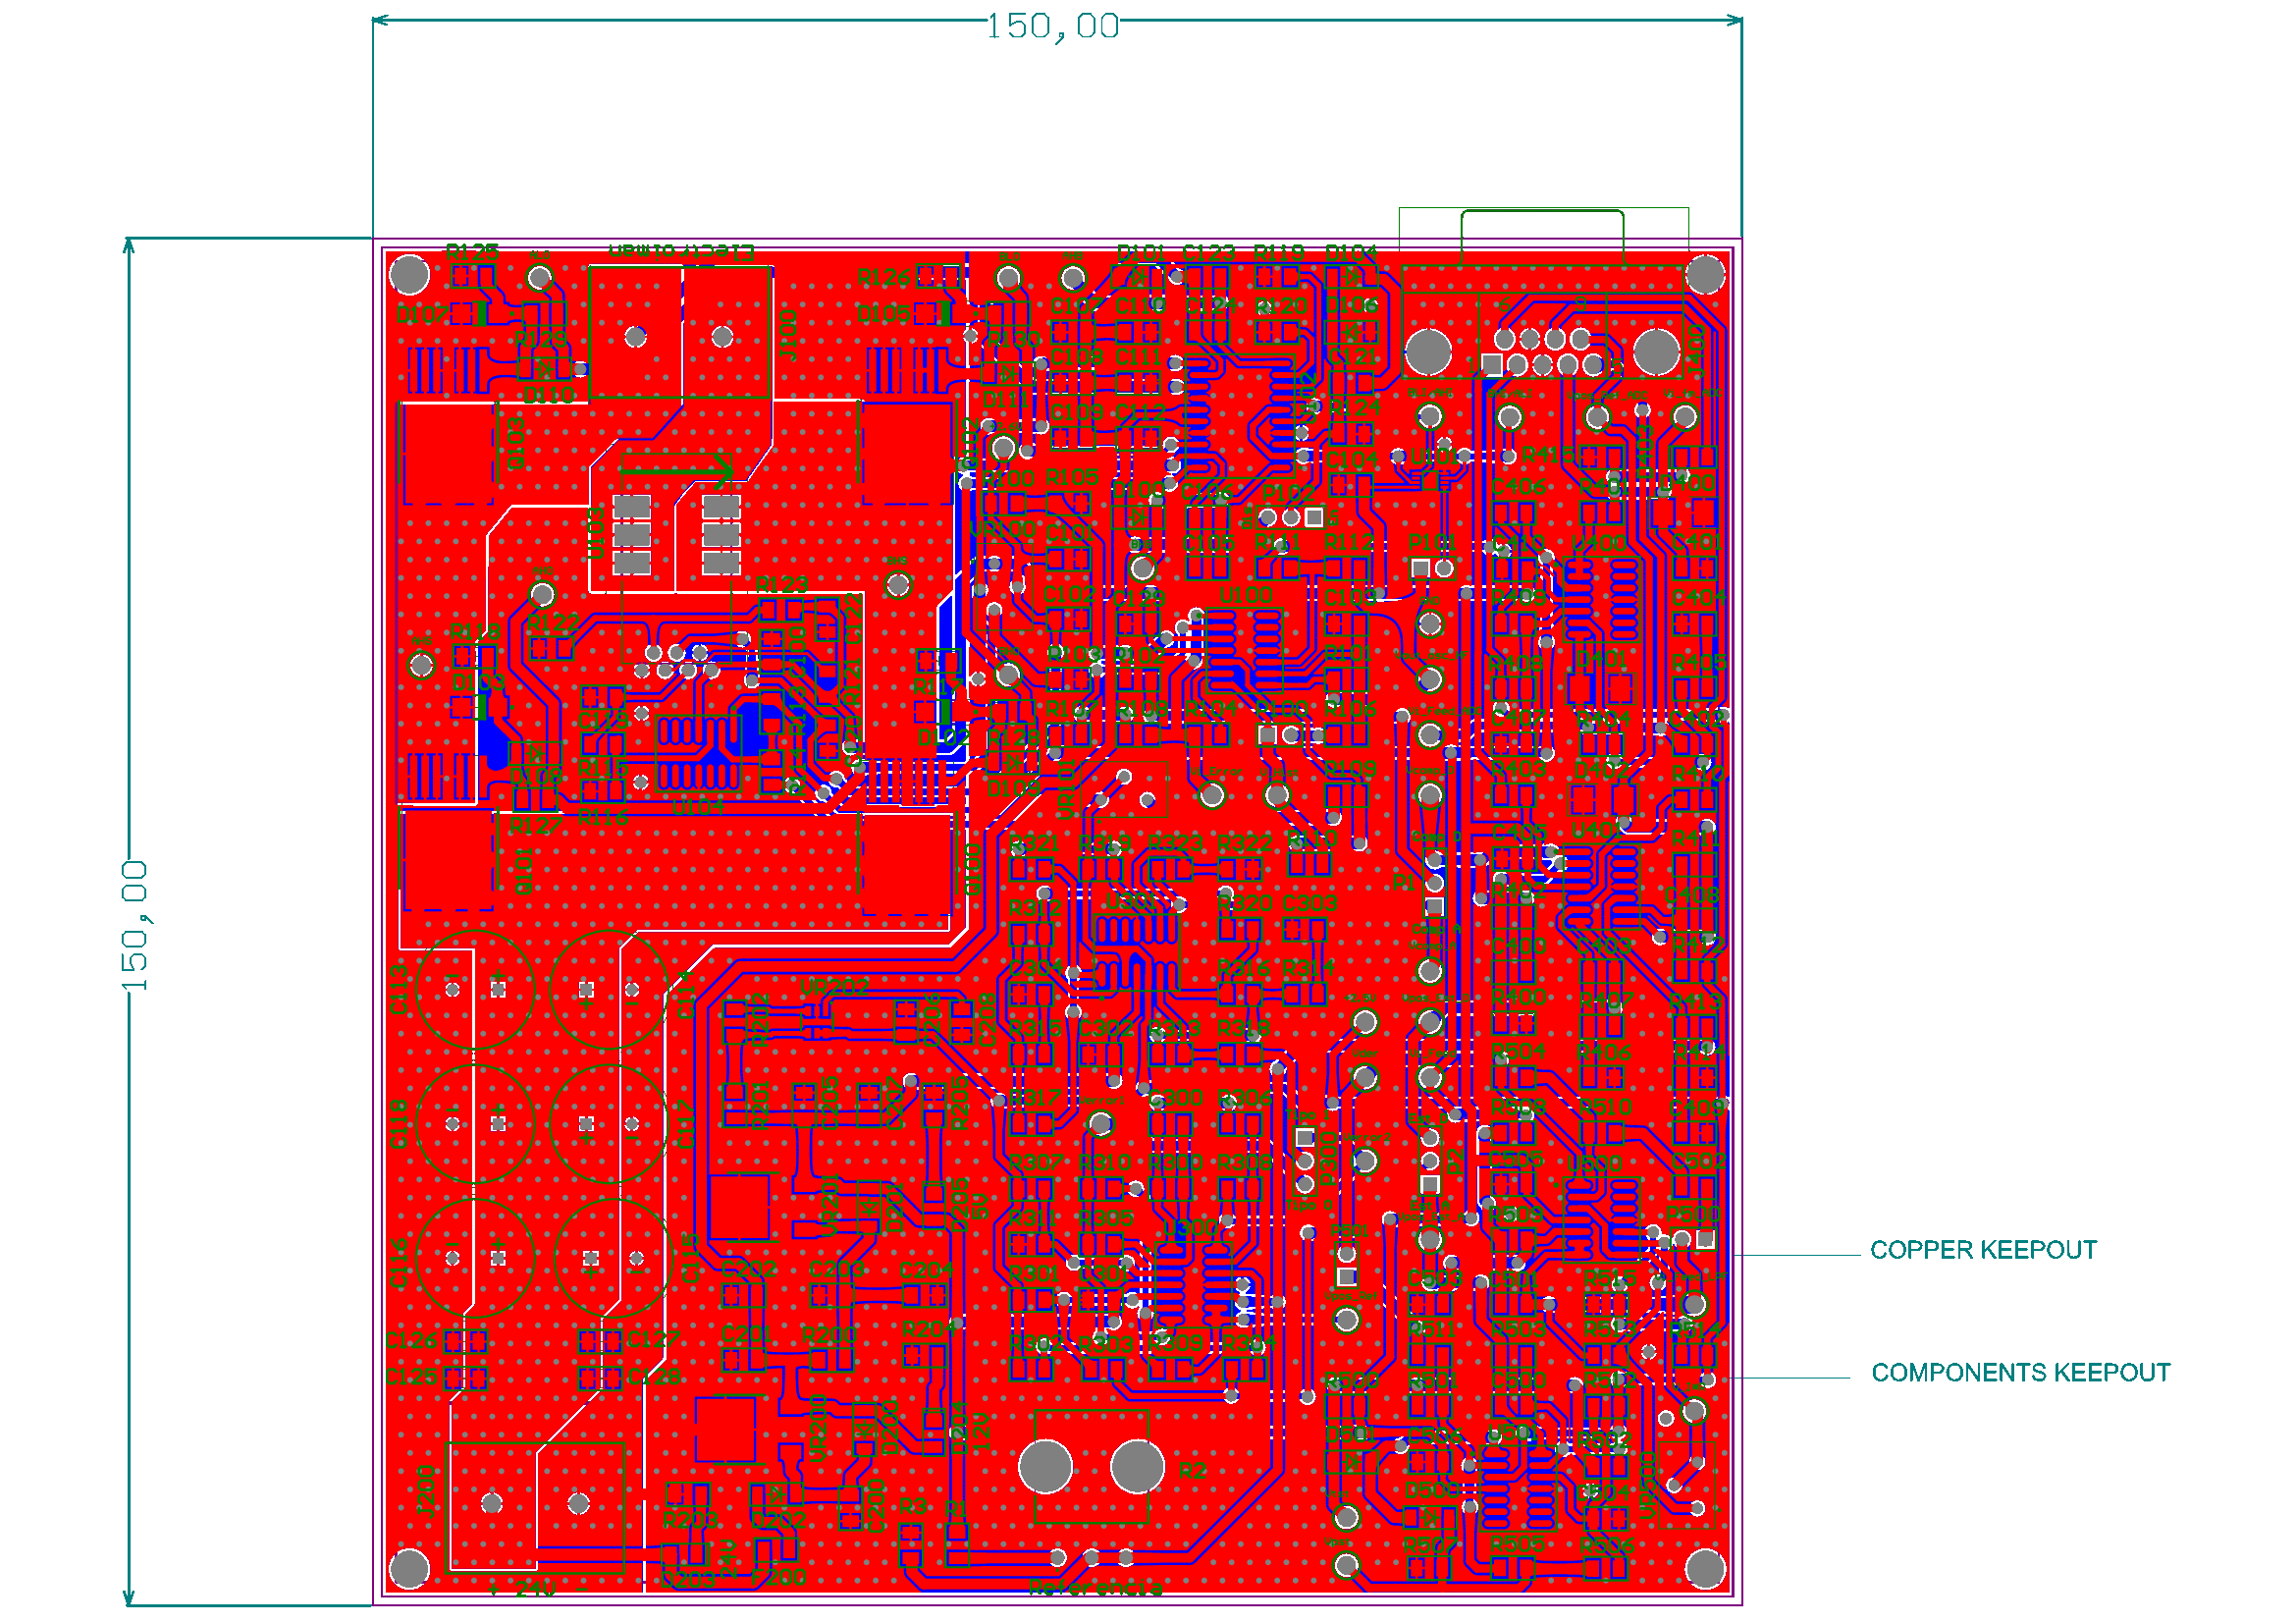
\includegraphics[scale=0.2]{VistSup.png}
	%\caption{Diagrama en bloques de la implementación digital.}
	\label{fig:VistSup}
\end{figure}

\subsubsection{Vista Inferior}
\begin{figure}[H]
	\centering
	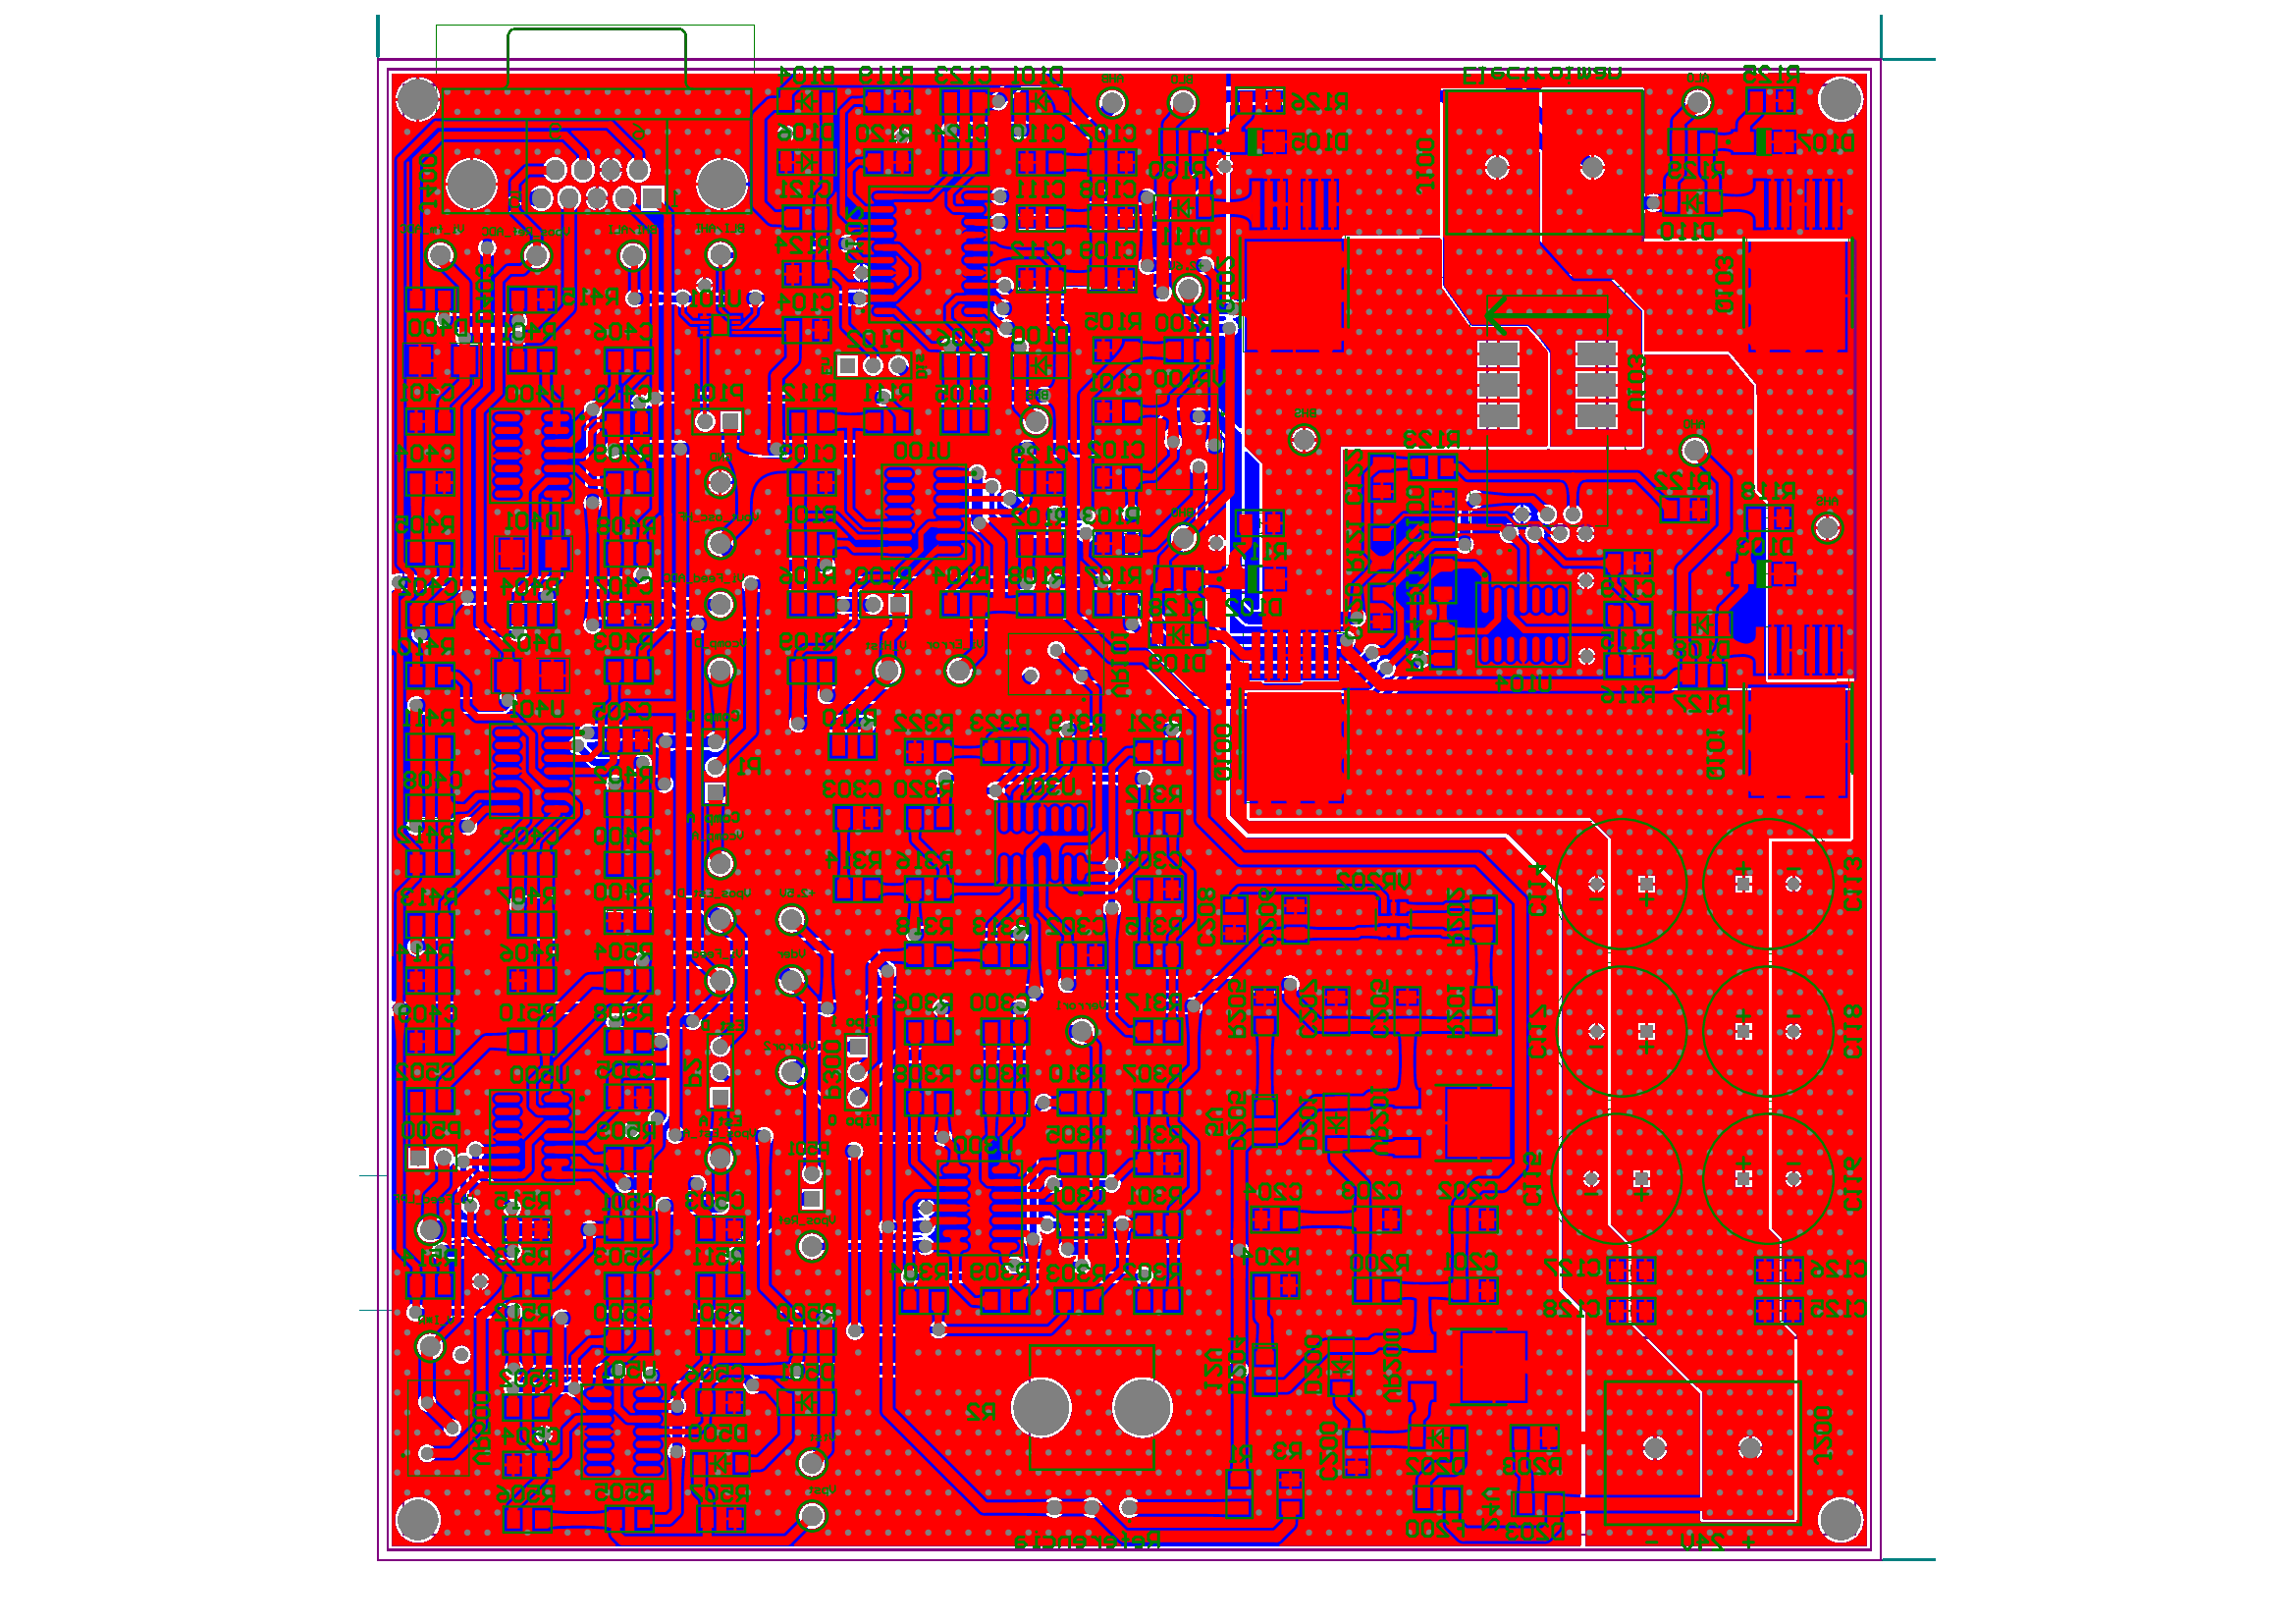
\includegraphics[scale=0.2]{VistInf.png}
	%\caption{Diagrama en bloques de la implementación digital.}
	\label{fig:VistInf}
\end{figure}

\subsection{Modelo 3D}
\subsubsection{Vista Superior}
\begin{figure}[H]
	\centering
	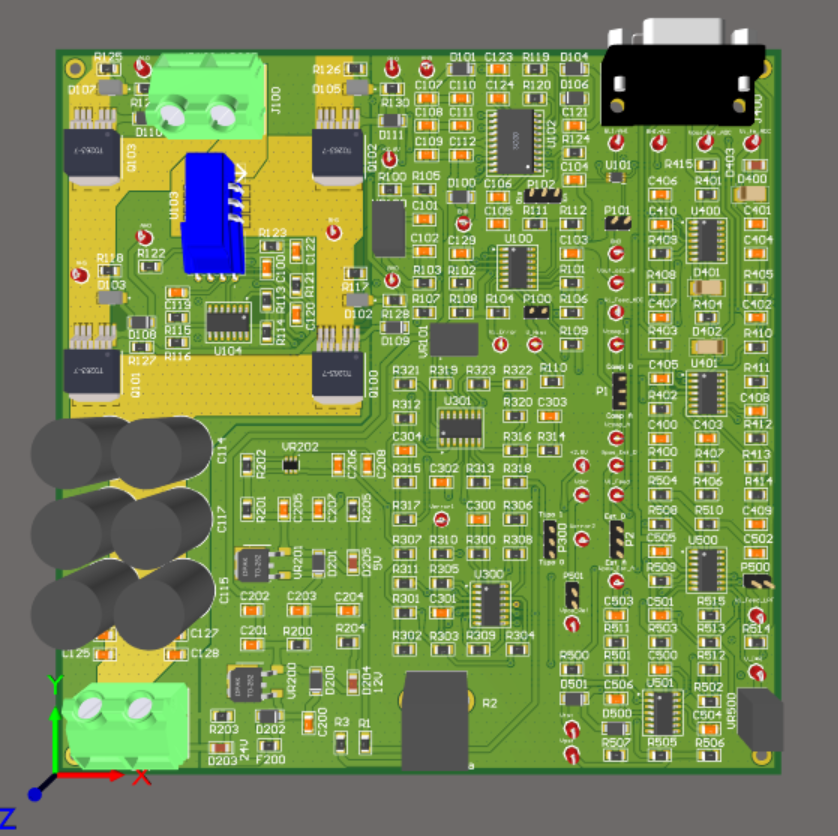
\includegraphics[scale=0.3]{VistSup3D.png}
	%\caption{Diagrama en bloques de la implementación digital.}
	\label{fig:VistSup3D}
\end{figure}

\subsubsection{Vista Inferior}
\begin{figure}[H]
	\centering
	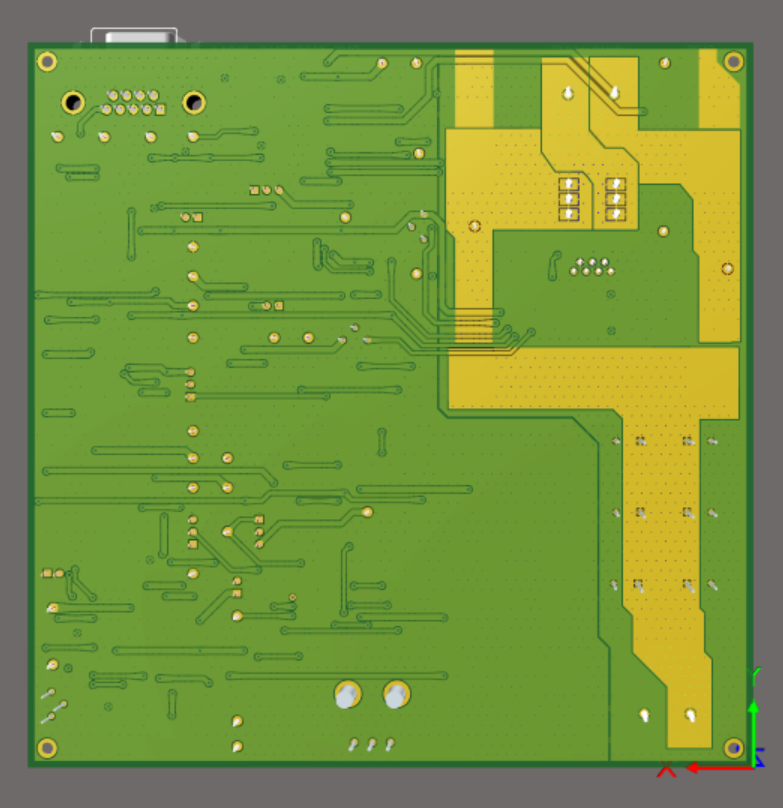
\includegraphics[scale=0.3]{VistInf3D.png}
	%\caption{Diagrama en bloques de la implementación digital.}
	\label{fig:VistInf3D}
\end{figure}

